\subsection{OpcuaServer}
%kurze Erwähnung sinn der klasse
%datenaustausch zwischen OpcuaServer zu abgeleitetrer...(dispatcher.... ) (I/O)
\begin{figure}[ht]
  \centering
  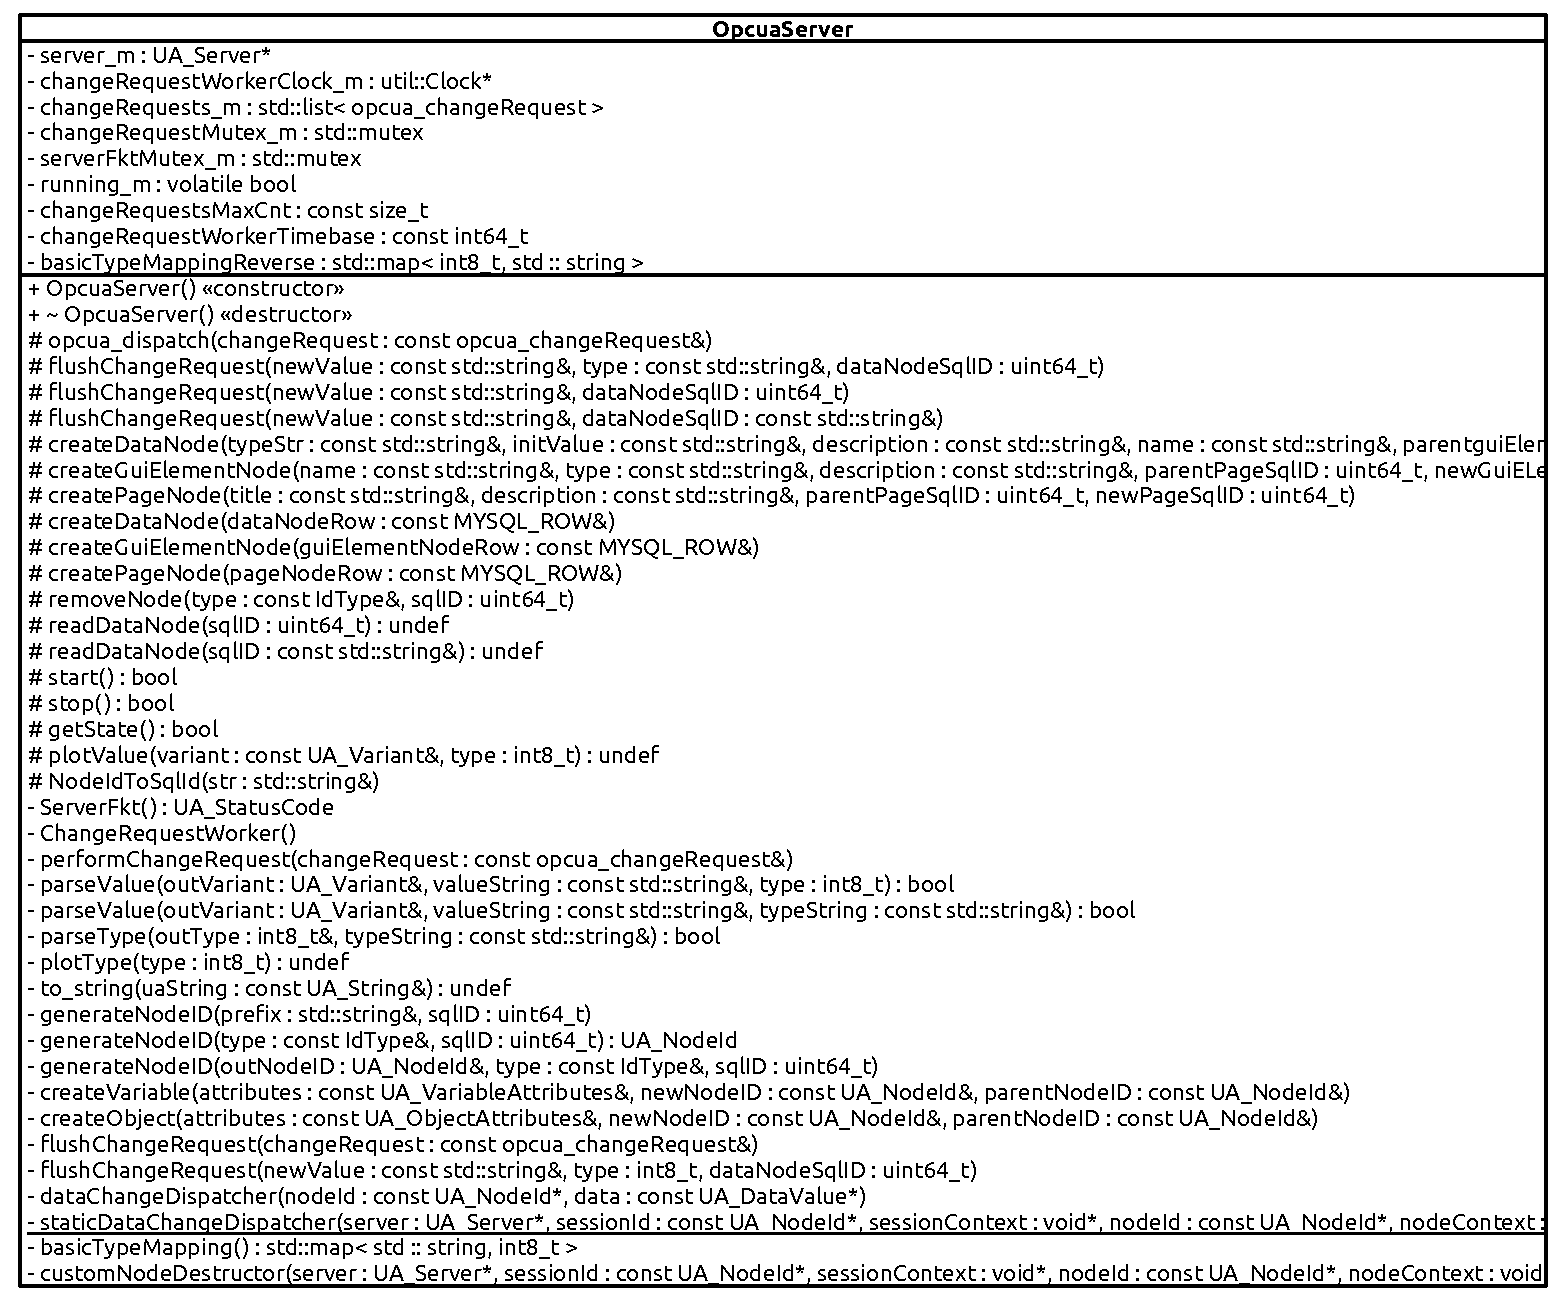
\includegraphics[width=\textwidth]{content/hauptteil/umsetzungPoC/backend/uml/classesOfOverview/OpcuaServer.pdf}
  \caption{Klassediagramm der Klasse \eigenName{OpcuaServer}}
  \label{fig:backend:classDiag:OpcuaServer}
\end{figure}
%beschreibung msg klasse mit diagram
\begin{figure}[ht]
  \centering
  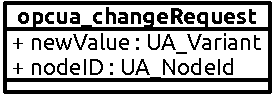
\includegraphics[width=0.2\textwidth]{content/hauptteil/umsetzungPoC/backend/uml/classesOfOverview/opcua_changeRequest.pdf}
  \caption{Klassediagramm der Klasse \eigenName{opcua\_changeRequest}}
  \label{fig:backend:classDiag:opcuaCR}
\end{figure}
%dispatcher codeausschnitt
%beschreibung dispatcher